\documentclass[tikz,svgnames]{standalone}

\usetikzlibrary{decorations.markings,positioning,decorations.pathmorphing}

\begin{document}
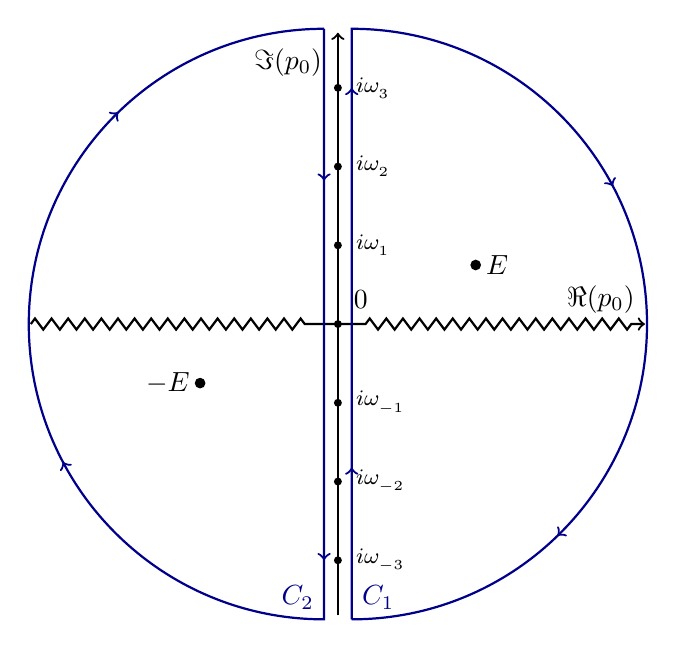
\begin{tikzpicture}[thick]

  \def\xr{3.5} \def\yr{3}

  % Axes
  \draw [decorate,decoration={zigzag,segment length=6,amplitude=2,post=lineto,post length=10}] (-\xr-0.4,0) -- (0,0);
  \draw [->,decorate,decoration={zigzag,segment length=6,amplitude=2,pre=lineto,pre length=10,post=lineto,post length=3}] (0,0) -- (\xr+0.4,0) node [above left]  {$\Re(p_0)$};
  \draw [->] (0,-\yr-0.7) -- (0,\yr+0.7) node[below left=0.1] {$\Im(p_0)$};

  % Matsubara frequencies
  \foreach \n in {-\yr,...,-1,1,2,...,\yr}{%
      \draw[fill] (0,\n) circle (1pt) node [right=0.1,font=\footnotesize] {$i \omega_{_{\n}}$};}
  \draw[fill] (0,0) circle (1pt) node [above right=0.1] {0};

  % Right contour line
  \draw[xshift=5,DarkBlue,decoration={markings,mark=between positions 0.1 and 1 step 0.25 with \arrow{>}},postaction={decorate}] (0,-\yr-0.75) node [above right] {$C_1$} -- (0,\yr+0.75) arc (90:-90:\yr+0.75);

  % Left contour line
  \draw[xshift=-5,DarkBlue,decoration={markings,mark=between positions 0.1 and 1 step 0.25 with \arrow{>}},postaction={decorate}] (0,\yr+0.75) -- (0,-\yr-0.75) node [above left] {$C_2$} arc (270:90:\yr+0.75);

  % Poles
  \draw[fill] (\xr/2,\yr/4) circle (1.5pt) node [right] {$E$};
  \draw[fill] (-\xr/2,-\yr/4) circle (1.5pt) node [left] {$-E$};

\end{tikzpicture}
\end{document}